% Copyright (c) 2014,2016 Casper Ti. Vector
% Public domain.

%\chapter{Nonstandard states}
%\pkuthssffaq % 中文测试文字。

\section{Derivation}
%The standard model is the theory that describe the basic forces between elementary particle in the universe, 

\subsection{The standard model}

In the field of paricle physics,
tremendous success have been achieved in standard model,
%the standard model has a excessive success,
which is a systematic theory 
that describes three known basic forces ( the electromagnetic, weak and strong interactions, except gravitaional force) and classifis all know elementary paricles.
As shown in Figure.~\ref{fig:standard_model},
there are two kinds of elementary paricles, 
one is called fermions with spin number equal to $1\slash2$, 
while the other is named as bosons with integral spin number.
The basic fermions include 6 quarks and 6 leptons, 
the quarks carry the color charge and interact via the strong interaction, 
which is described by quantum chromodynamics (QCD), 
more details about this theory will be discussed later.
Leptons can participate the weak and electromagnetic forces,
and the electroweak sector is described by gauge theory with the symmetry group $\mbox{U}(1) \times \mbox{U}(2)$.

\begin{figure}[!hbtp]
\centering
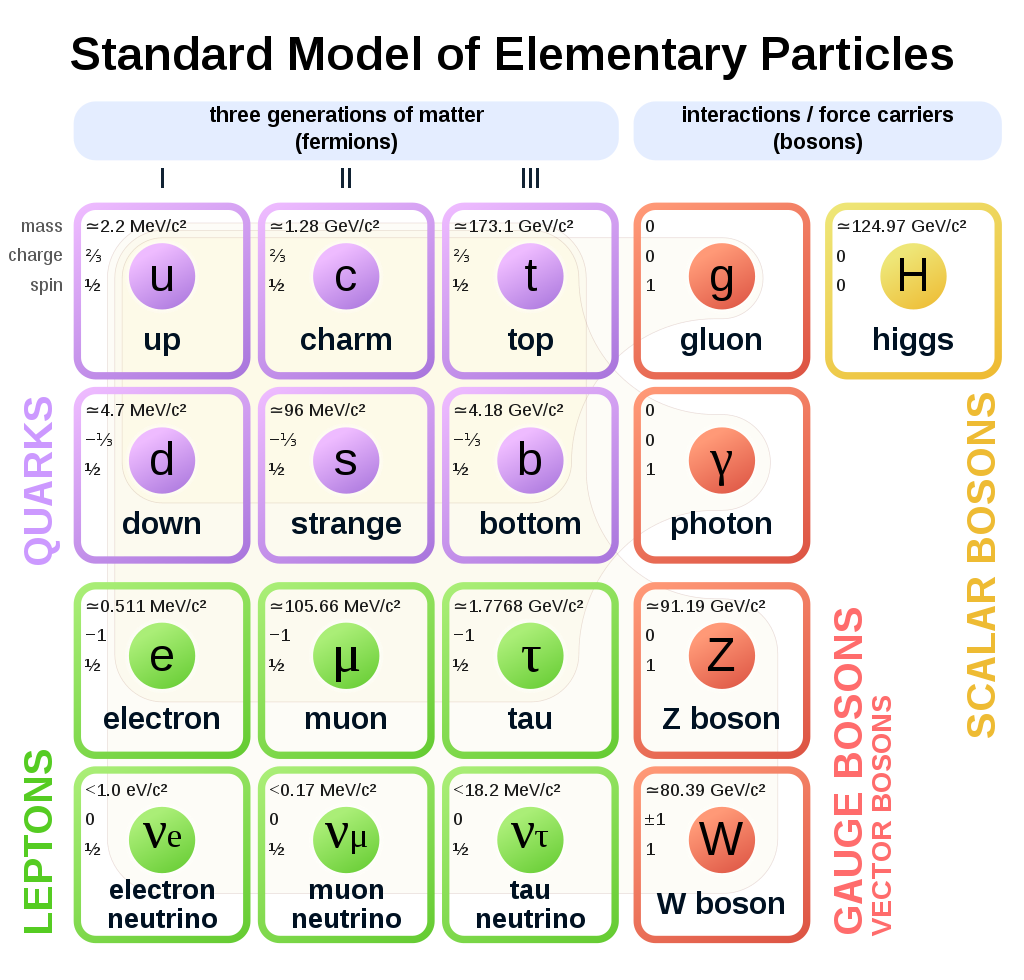
\includegraphics[width=0.55\textwidth]{Figures/01_Introduction/Physics/Standand_model.png}%
\caption{The elementary particle in the standard model.}
\label{fig:standard_model}
\end{figure}


%\textcolor{red}{Discuss more ??? and some texts connecting above and below. }


\subsection{Quark model and QCD}

%\textcolor{red}{Breif history of quark model}

Circa 1950,
the first particle accelerator began to uncover many new particles,
and most of these particles are unstable and decay very quickly,
and hence had not been seen in cosmic ray experiment,
as shown in the Figure.~\ref{fig:particle_zoo}.
With the particle "Zoo" proliferation, 
people suspected that if all these particles are fundamental, 
and W. Lamb joked that he had heard it said that 
"the finder of a new elementary particle used to be rewarded by a Nobel Prize, 
but such a discovery now ought to be punished by a \$10,000 fine."\supercite{Lamb439}
The prosperity of new particles observed from experiments promoted emergence of many new models,
which concocted to try to explain why these particles exit,
such as,
the model of pion composed of nucleons and anti-nucleons from Fermi and Yang\supercite{PhysRev.76.1739},
which was proposed before the discovery of anti-proton.
The quark model was constructed in the early 1960s by M. Gell-Mann and G. Zweig independently to classify scheme for hadrons \supercite{GellMann:1964nj, Zweig:570209},
which gives a natural explanation for isospin and strangeness.
Besides, 
this model predicted the existence of the spin $-3\slash2$ \Omegam,
which is a member of the ground-state decuplet,
and the observation for the this paricle offered a strong evidence of correction of quark model \supercite{PhysRevLett.12.204}.

\begin{figure}[!hbtp]
\centering
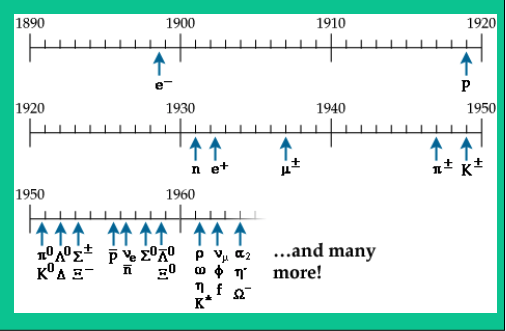
\includegraphics[width=0.65\textwidth]{Figures/01_Introduction/Physics/Particle_Zoo.png}%
\caption{The particle zoo before 1964.}
\label{fig:particle_zoo}
\end{figure}

\subsubsection{Quark model}

The quark model is a description of hadronic properties which strongly emphasizes the role of the minimum-quark-content part of the wave function of hadron\supercite{PDG2020}.
In this model, 
the quarks are strongly interacting fermions with spin $1\slash2$ and positive parity,
while the antiquarks have nagetive parity.
The Table~\ref{tab:quantum_quarks} lists all quantum number of 6 kinds of quarks.
All of them are related with each other through the generalized Gell-Mann-Nishijima formualr:
\begin{equation}
Q = I_z + \frac{\BR + S + C + B + T}{2}
\label{eq:GMN_equation}
\end{equation}
This convension imply the charged meson has the same sign as its charge.
Besides, 
the hypercharge is another useful quantum number, 
which is defined as:
\begin{equation}
	Y = \BR + S -  \frac{C - B + T}{3}
\label{eq:GMN_equation_2}
\end{equation}


\begin{table}[h]
\caption{Some quantum numbers of quarks.}
\begin{center}
	\begin{tabular}{c| cccccc}
\hline \hline
    						&   \dquark  		&  \uquark   		& \squark  			&  \cquark   		&  \bquark   		&   \tquark  \\
\hline 
$Q$(electric charge)   		&   $-\frac{1}{3}$  &   $+\frac{2}{3}$  &   $-\frac{1}{3}$  &   $+\frac{1}{3}$  &   $-\frac{1}{3}$  &   $+\frac{1}{3}$      \\
$I$(isospin)   				&   $\frac{1}{2}$   &   $\frac{1}{2}$   &   $0$ 			&   $0$  			&   $0$  			&   $0$      \\
$I_z$(isospin z-componet) 	&   $\frac{1}{2}$   &   $-\frac{1}{2}$  &   $0$  			&   $0$  			&   $0$  			&   $0$      \\
$S$(strangness)   			&   $0$  			&   $0$  			&   $-1$  			&   $0$  			&   $0$  			&   $0$      \\
$C$(charm)   				&   $0$  			&   $0$  			&   $0$  			&   $+1$  			&   $0$  			&   $0$      \\
$B$(bottomness)   			&   $0$  			&   $0$  			&   $0$  			&   $0$  			&   $-1$  			&   $0$      \\
$T$(topness)   				&   $0$  			&   $0$  			&   $0$  			&   $0$  			&   $0$  			&   $+1$      \\
\BR(baryon)   				&   $\frac{1}{3}$  	&   $\frac{1}{3}$  	&   $\frac{1}{3}$  	&   $\frac{1}{3}$  	&   $\frac{1}{3}$  	&   $\frac{1}{3}$      \\
\hline \hline
\end{tabular}
\normalsize
\label{tab:quantum_quarks}
\end{center}
\end{table}

Quarks are added together to form mesons and baryons using SU(3) group,
and mesons are bound states of quark-antiquark, 
while the baryons are bound states of three quarks.
The properitis of SU(3) tell us the number of the multiplets belonging to product of 3 by 3:
\begin{equation}
	3 \otimes \bar{3} = 1 \oplus 8
\label{eq:meson_3}
\end{equation}
If a fourth quark such as charm \cquark included, 
the SU(3) group can be extended to SU(4), 
and the sixteen mesons are grouped into a 15-plet and a singlet:
\begin{equation}
	4 \otimes \bar{4} = 1 \oplus 15
\label{eq:meson_4}
\end{equation}
And this model can be extended with \bquark included naturally.


The diagram of meson model is very clear and simple, 
and the similar picture can also be extended to baryons.
The "ordinary" baryons are composed of \uquark, \dquark and \squark quarks,
which can be processed in a similar manner to combine three triplets,
namely three representations:
\begin{equation}
	3 \otimes 3 \otimes 3 = 10_{s} \oplus 8_{M,S} \oplus 8_{M,A} \oplus 1_{A}
\label{eq:baryon_3}
\end{equation}
Here $10_{S}$ means symmetric states, 
$8_{M,S}$ and $8_{M,A}$ are mixed symmetry and anti-symmetry combinations respectively,
and $1_{A}$ is a completely anti-symmetric three-quark system,
where the symmetries referred to are under the exchange of any two quarks.


\subsubsection{QCD}

The quark model successfully accommodates all these particles and resonances.
A remarkable success of the $SU(3)_f$ was the prediction, 
including the mass of the $M(\Omegam)=\squark\squark\squark$ baryon\supercite{PhysRevLett.12.204}.
But the model has following problems.
First, 
the most obvious problem is that no matter how hard physicists have tried, 
a free quark has never been observed.
Is the quark a real particle or simply a methematical construct that allows us to keep track to $SU(3)_f$ in an efficient manner.
The second problem is the absence of anti-symmetric combinations of spin and of flavour representations in the baryon sector.
This is not unrelated to a third problem, 
that of Fermi-Dirac statistics.
Baryons, having an odd number of spin-$\frac{1}{2}$ components, 
should have totally anti-symmetric wave-funcitons.
Since they have $L=0$,
their spatial wave-function is symmetric,
and we have imposed that their spin and flavour wave-function factors be symmetric too.
Therefore,
the wave-functions are totally symmetic.

To solve the Fermi-Dirac statistic problem, 
Han and Nambu, Greenberg and Gell-Mann, 
independently proposed adding an additional quantum number to the quarks, 
which is named as "color"\supercite{}.
The Lagrangian of QCD is given by:
\begin{equation}
	\lum = \sum_{q}{\bar{\psi}_{q,a}(i\gamma^{\mu}\partial_{\mu}\delta_{ab}
	-g_{s}\gamma^{\mu}t_{ab}^C}\mathcal{A}_{\mu}^{C}
	-m_{q}\delta_{ab})\psi_{q,b}
	-\frac{1}{4}F_{\mu\nu}^{A}F^{A \mu\nu} 
\label{eq:baryon_3_2}
\end{equation}
where the repeated indices are summed over.
The $\gamma^{\mu}$ are the Dirac $\gamma$-matrixs.
The $\psi_{q,a}$ are quark-field spinors for a quark of flavour $q$ and mass $m_{q}$,
with a color-index $a$ that runs from 1 to 3.
Quarks are said to be in the fundamental representation of the SU(3) color group.
The $\mathcal{A}_{\mu}^{C}$ is the gluon fields,
with $C$ running from 1 to 8,
corresponding to eight kinds of gluon.
The $t_{ab}^C$ represents eight $3\times3$ matrixes and are the generators of SU(3) group,
which illuminates the fact that a gluon's interaction with quark rotates the quark's color in SU(3) space.
The quantity $g_s$ is the QCD coupling constant.
Neither quarks nor gluons are observed as free particles.
Hadrons are color-singlet combination of quarks, anti-quarks, and gluons.
From above formula, 
the fundamental parameters of QCD are the coupling $g_s$ and the quark masses $m_q$.


\begin{figure}[!hbtp]
\centering
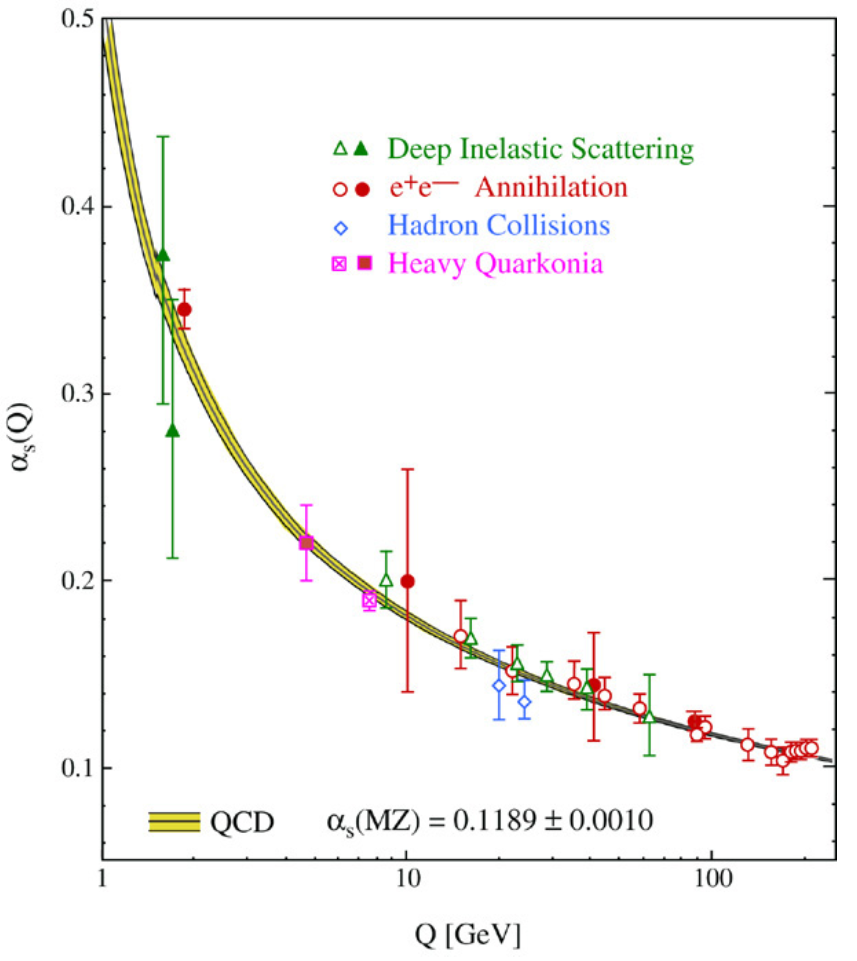
\includegraphics[width=0.45\textwidth]{Figures/01_Introduction/Physics/QCD_asymptotic.png}%
	\caption{Summary of measurements of $\alpha_{s}(Q)$ as a function of hte respective energy scale Q. 
	Figure taken from Ref.~\cite{BETHKE2007351}}
\label{fig:QCD_asymptotic}
\end{figure}


Another intersting phenomenon in QCD is asymptotic freedom,
which leads to a consequence that the strong coupling $\alpha_{s}$ is small enough,
as sufficiently large momentum transfers,
to allow application of perturbation theory in order to provide quantitaive predictions of physical processes.
The strong interaction coupling constant $\alpha_s$ is fundamentally different from the quantum electrodynamics coupling constant,
as not only fermion loops are included in the vertex expansion, 
but also gluon loops, 
owing to the fact that the gluon carry colour charges.
And in QCD,
the gluon-gluon interaction includes additional vacuum polarization diagrams that have virtual gluon loops.
These gluon loops modify the QCD coupling strength $\alpha_s$ in a way that is opposite to QED:
they cause $\alpha_s$ to decrease at short distances and increase at long distances, as shown in Figure.~\ref{fig:QCD_asymptotic} 

%\textcolor{red}{I am not sure if necessary to review more on basic theory. }


\subsubsection{The QCD dilemma}
In QCD,
the component of the standard model of elementary processes that deal with strong interaction,
the elementary particles are color-charged quarks and gluons.
However,
a consequence of confinement is that these particles cannot be seen in experiments.
Although the QCD Lagrangian is expected, 
in priciple,
to completely describe the spectrum of hadrons and all of their properities,
there is no rigorous first-principle translation of this into any useful mathematical expressions.

A fundamental process that can be computed with perturbative QCD is quark-quark elastic scattering at high-momentum transfer.
This shows up in high-energy $pp$ collider experiments as events with two high transverse momentum jets of hadrons 
that are nearly back to back in azimuth. 
The momentum distribution of quarks inside the proton is governed by long-distance QCD 
and approximated by universal parton distribution functions
that are taken from fits to data obtaind from hadron-collider measurements at low center of mass energies,
deep inelastic lepton-proton scattering experiments, etc.
The fundamental QCD $pp\to pp$ process cannot be directly measured,
instead, 
have to be inferred from the jets of hadrons that they produce.
Thus,
even processes that are perturbative QCD calculations involve significant long-distance QCD effects both in the inital and final states.

This nearly total disconnect between the hadrons observed in experiments and the quarks and gluons 
that appear in the theory is a problem of large proportions in paritcle physics.
This is refered as "QCD dilemma".
In addition to the intellectual dissatisfaction with a theory that is not directly applicable to the particles used and detected in experiments,
there is also a practical problem in that many SM tests and searches for new physics (NP) with strong interacting hadrons involved 
in the initial and final states of the associated measurements.
Even experiments without initial or final states that contain hadrons are still subject to their effects from virtual quantum fluctuations.
As a result,
the sensitivities of many NP searching experiments are ultimately limited by hadron-related theoretical uncertainties.
Because of this,
as the experimental sensitivities of NP searches improve,
commensurate improvements of long-distance QCD become more and more important.


A possible way experiments might contribute to these improvements is by identifying patterns in hadron physics
that may help guide the development of improved theoretical models,
and the multi-quark states study offers an unique method to probe QCD. 


\subsection{Multiquark states}

The concept of multiquark resonances came out accompanying with the quark model, 
as G. Zweig\supercite{Zweig:570209} said: 
{\slshape"In general, we would expect that baryons are built not only from product of these aces, 
$AAA$, but also from $\bar{A}AAAA$, 
$\bar{A}\bar{A}AAAAA$", \etc,
where $\bar{A}$ denotes an anti-ace."}
and M. Gell-Mann\supercite{GellMann:1964nj} gave the similar expression:
{\slshape"Baryons can now be constructed from quarks by using the combinations ($qqq$), ($qqqq\bar{q}$), \etc,
while mesons are made of ($q\bar{q}$), ($qq\bar{q}\bar{q}$, \etc)"}.
By then,
many experiments tried to search tetraquark and pentaquark states,
for example,
LEPS Collaboration declared the observation of a narrow $\Theta^{+}(1540)$ paricle,
which is claimed as a pentaquark candidates,
then this state became a hotspot at that time.\supercite{PhysRevLett.91.012002,doi:10.1142/S0217751X04019676}
However, 
this structure was not confirmed from high precise experiments \supercite{doi:10.1142/S0217751X14300208},
and it is not deemed as a genuine resonance now \supercite{PhysRevLett.105.092001}.
The research to $\Theta^{+}(1540)$ told us lessons but also brought us precious experience and opportunities,
so we should not ignore the non-perturbative chromodynamics in spectroscopy study.

A bit of history is mentioned above, 
and current progress about heavy-flavour multiquark study will be reviewed from two perspectives,
experimental evidences and theoretical models in next sections.

%\begin{figure}[!hbtp]
%\centering
%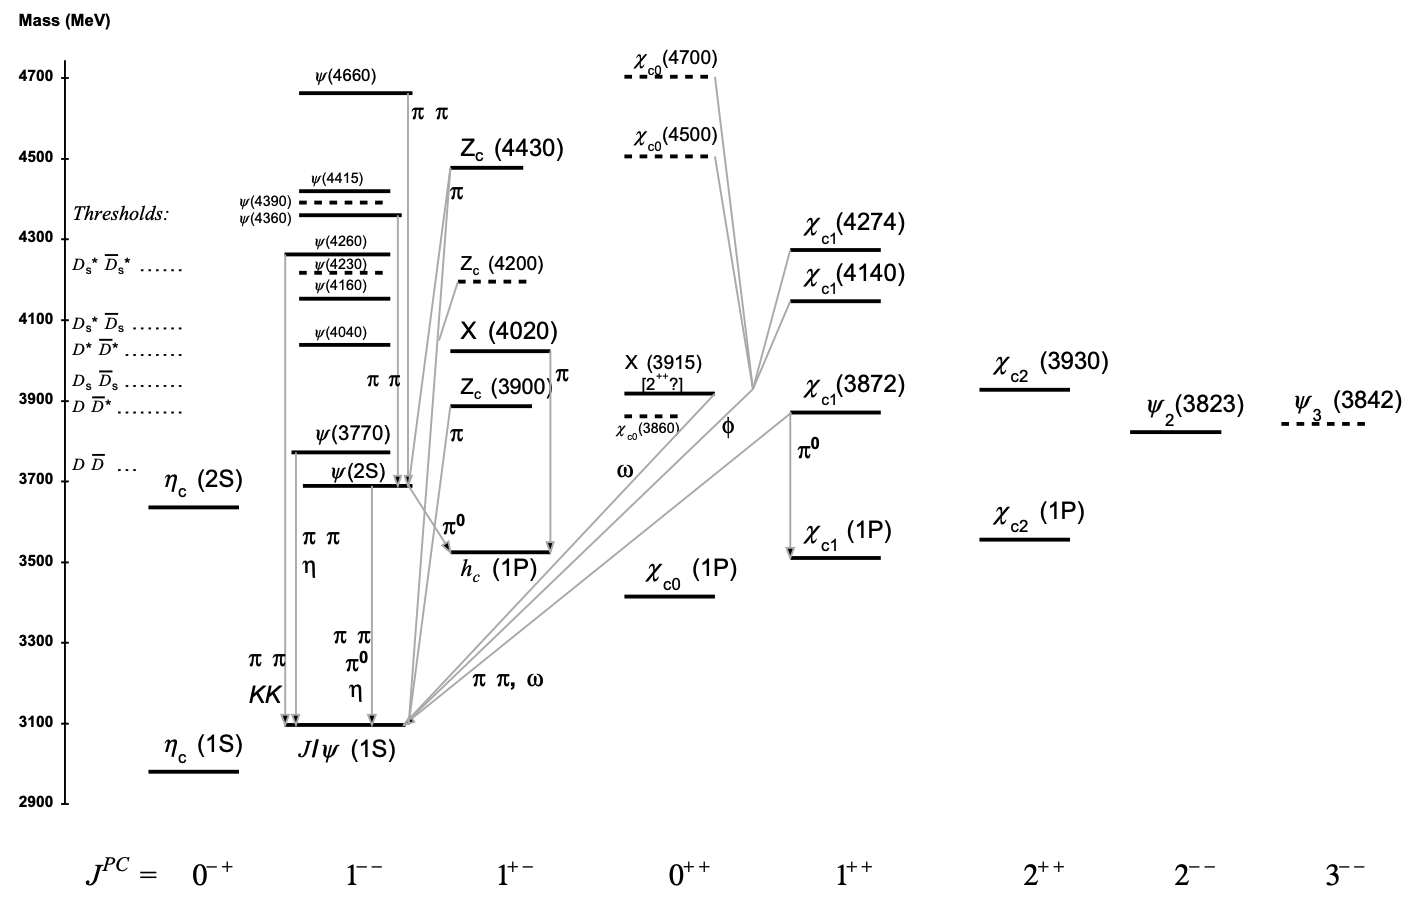
\includegraphics[width=0.8\textwidth]{Figures/01_Introduction/Exotic/charmonium_spect.png}%
%\caption{The level scheme of meson states containing a minimal quark content \cquark\cquarkbar. 
%         The name of a state is determined by its quantum number $I^{G}J^{PC}$.
%	   The arrows indicate the most dominate hadronic transitions.
%	   Taken from Ref.~[\cite{PDG2020}].}
%\label{fig:Charmonium_PDG}
%\end{figure}

The obseverd status of the charmonium-like spectrum are listed in Figure.~\ref{fig:Charmonium_Mod},
which includes the standard charmonium,
non-standard charmonium (tetraquark candidates) and pentaquark candidates.
%The non-standard states have possibility making up of more than two quarks,
%which is also taken as tetraquark candidates.
{\color{red} Maybe to update later, to include 3$P_{c}$, $Z_{cs}$, $T_{cccc}$ and new $X$.}

\begin{figure}[!hbtp]
\centering
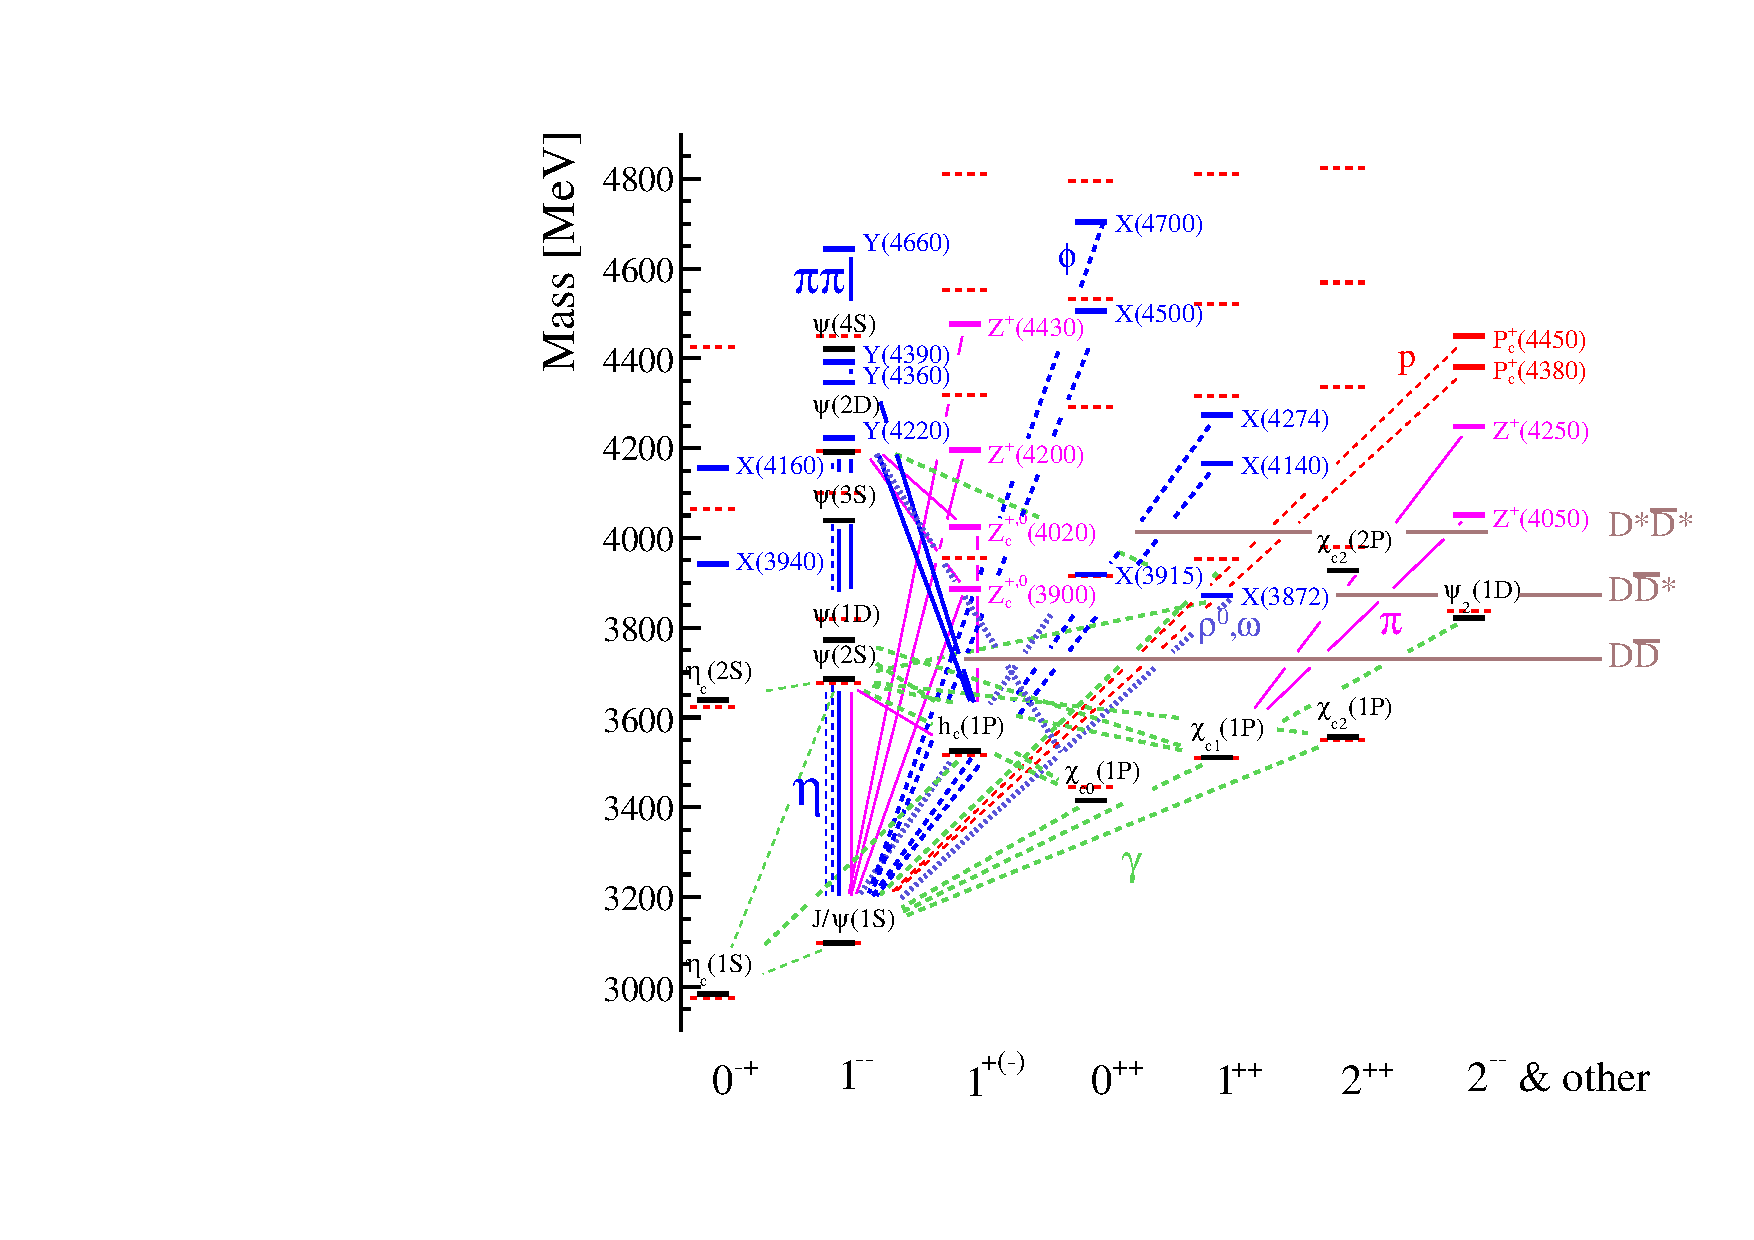
\includegraphics[width=0.8\textwidth]{Figures/01_Introduction/Exotic/charmoniumExotic}%
\caption{The level scheme of meson states containing a minimal quark content \cquark\cquarkbar. 
         The name of a state is determined by its quantum number $I^{G}J^{PC}$.
	   The arrows indicate the most dominate hadronic transitions.
	   Taken from Ref.~[\cite{RevModPhys.90.015003}].}
\label{fig:Charmonium_Mod}
\end{figure}






